
 
\documentclass[11pt,compress,t,notes=noshow]{beamer}

\usepackage[english]{babel}
\usepackage{dsfont}
\newcommand\bmmax{2}
\usepackage{bm}
\usepackage{bbm}
\usepackage{verbatim}
\usepackage{amsmath}
\usepackage{amsfonts}
\usepackage{csquotes}
\usepackage{multirow}
\usepackage{longtable}
\usepackage{enumerate}
\usepackage[absolute,overlay]{textpos}
\usepackage{psfrag}
\usepackage{algorithm}
\usepackage{algorithmicx}
\usepackage{algpseudocode}
\usepackage{eqnarray}
\usepackage{multimedia}
\usepackage{media9}
\usepackage{arydshln}
\usepackage{tabularx}
\usepackage{placeins}
\usepackage{tikz}
\usepackage{setspace}
\usepackage{wrapfig}
\usepackage{tcolorbox}
\usepackage[export]{adjustbox}
\usepackage{siunitx}
\usetikzlibrary{shapes,arrows,automata,positioning,calc}
\tikzset{
  %Define standard arrow tip
  >=stealth',
  %Define style for boxes
  punkt/.style={
    rectangle,
    rounded corners,
    draw=black, very thick,
    text width=6.5em,
    minimum height=2em,
    text centered},
  % Define arrow style
  pil/.style={
    ->,
    thick,
    shorten <=2pt,
    shorten >=2pt,}
}
\usepackage{subfig}

%new environments

\newenvironment{vbframe}  %frame with breaks and verbatim
{
 \begin{frame}[containsverbatim,allowframebreaks]
}
{
\end{frame}
}

\newenvironment{vframe}  %frame with verbatim without breaks (to avoid numbering one slided frames)
{
 \begin{frame}[containsverbatim]
}
{
\end{frame}
}

\newenvironment{blocki}[1]   % itemize block
{
 \begin{block}{#1}\begin{itemize}
}
{
\end{itemize}\end{block}
}

\newenvironment{fragileframe}[2]{  %fragile frame with framebreaks
\begin{frame}[allowframebreaks, fragile, environment = fragileframe]
\frametitle{#1}
#2}
{\end{frame}}


\newcommand{\myframe}[2]{  %short for frame with framebreaks
\begin{frame}[allowframebreaks]
\frametitle{#1}
#2
\end{frame}}

\newcommand{\remark}[1]{
  \textbf{Remark:} #1
}

%%%%%%%%%%%%%%%%%%%%%%%%%%%%%%%%%%%%%%%%%%%%%%%%%%%%%%%%%%%%%%%%%%%%%%%%%%%%%%%

% basic latex stuff
\newcommand{\pkg}[1]{{\fontseries{b}\selectfont #1}} %fontstyle for R packages
\newcommand{\lz}{\vspace{0.5cm}} %vertical space
\newcommand{\dlz}{\vspace{1cm}} %double vertical space
\newcommand{\oneliner}[1] % Oneliner for important statements
{\begin{block}{}\begin{center}\begin{Large}#1\end{Large}\end{center}\end{block}}


%\usetheme{lmu-lecture}
\usepackage{../style/lmu-lecture}

\let\code=\texttt
\let\proglang=\textsf

\setkeys{Gin}{width=0.9\textwidth}



\title{Deep Learning}
\author{David Rügamer}
\institute{Department of Statistics -- LMU Munich}
\date{Winter Semester 2021}

\setbeamertemplate{frametitle}{\expandafter\uppercase\expandafter\insertframetitle}

%\begin{document}
%\sloppy
%\end{document}


\input{../../latex-math/basic-math}
\input{../../latex-math/basic-ml}
\input{../../latex-math/ml-nn}

\begin{document}

\lecturechapter{1}{Introduction to Deep Learning}
\lecture{Deep Learning}

%%%%%%%%%%%%%%%%%%%%%%%%%%%%%%%%%%%%%%%%%%%%%%%%%%%%%%%%%%%%%%%%%%

\begin{vbframe}
\frametitle{Lecture Outline}
\tableofcontents
\end{vbframe}


\section{Teaching Team}

\begin{frame}  {Dr. David R{\"u}gamer}

 I am Researcher and Lecturer at the Chair of Statistical Learning and Data Science.
    \begin{itemize}
      \item Ph.D. in Statistics with focus on Functional Data Analysis, Gradient Boosting and Statistical Inference. 
      \item M.Sc. in Statistics with Specialization in Theory
      \item B.Sc. in Statistics with a Minor in Computer Science
    \end{itemize}
    
  \begin{figure}
      \scalebox{0.25}{\includegraphics{plots/david.jpg}}

  \end{figure}
  
\end{frame}


\begin{frame}  {Mina Rezaei, Ph.D.}

 I am Researcher at the Chair of Statistical Learning and Data Science.
    \begin{itemize}
      \item Ph.D. in Computer Science with focus on Deep Representation Learning from Imbalanced/Long-tailed Data.
      \item M.Sc. in Artificial Intelligence with Machine Learning Application in Medical Image Diagnosis
      \item B.Sc. in Computer Science
    \end{itemize}
  \begin{figure}
    \centering
      \scalebox{0.25}{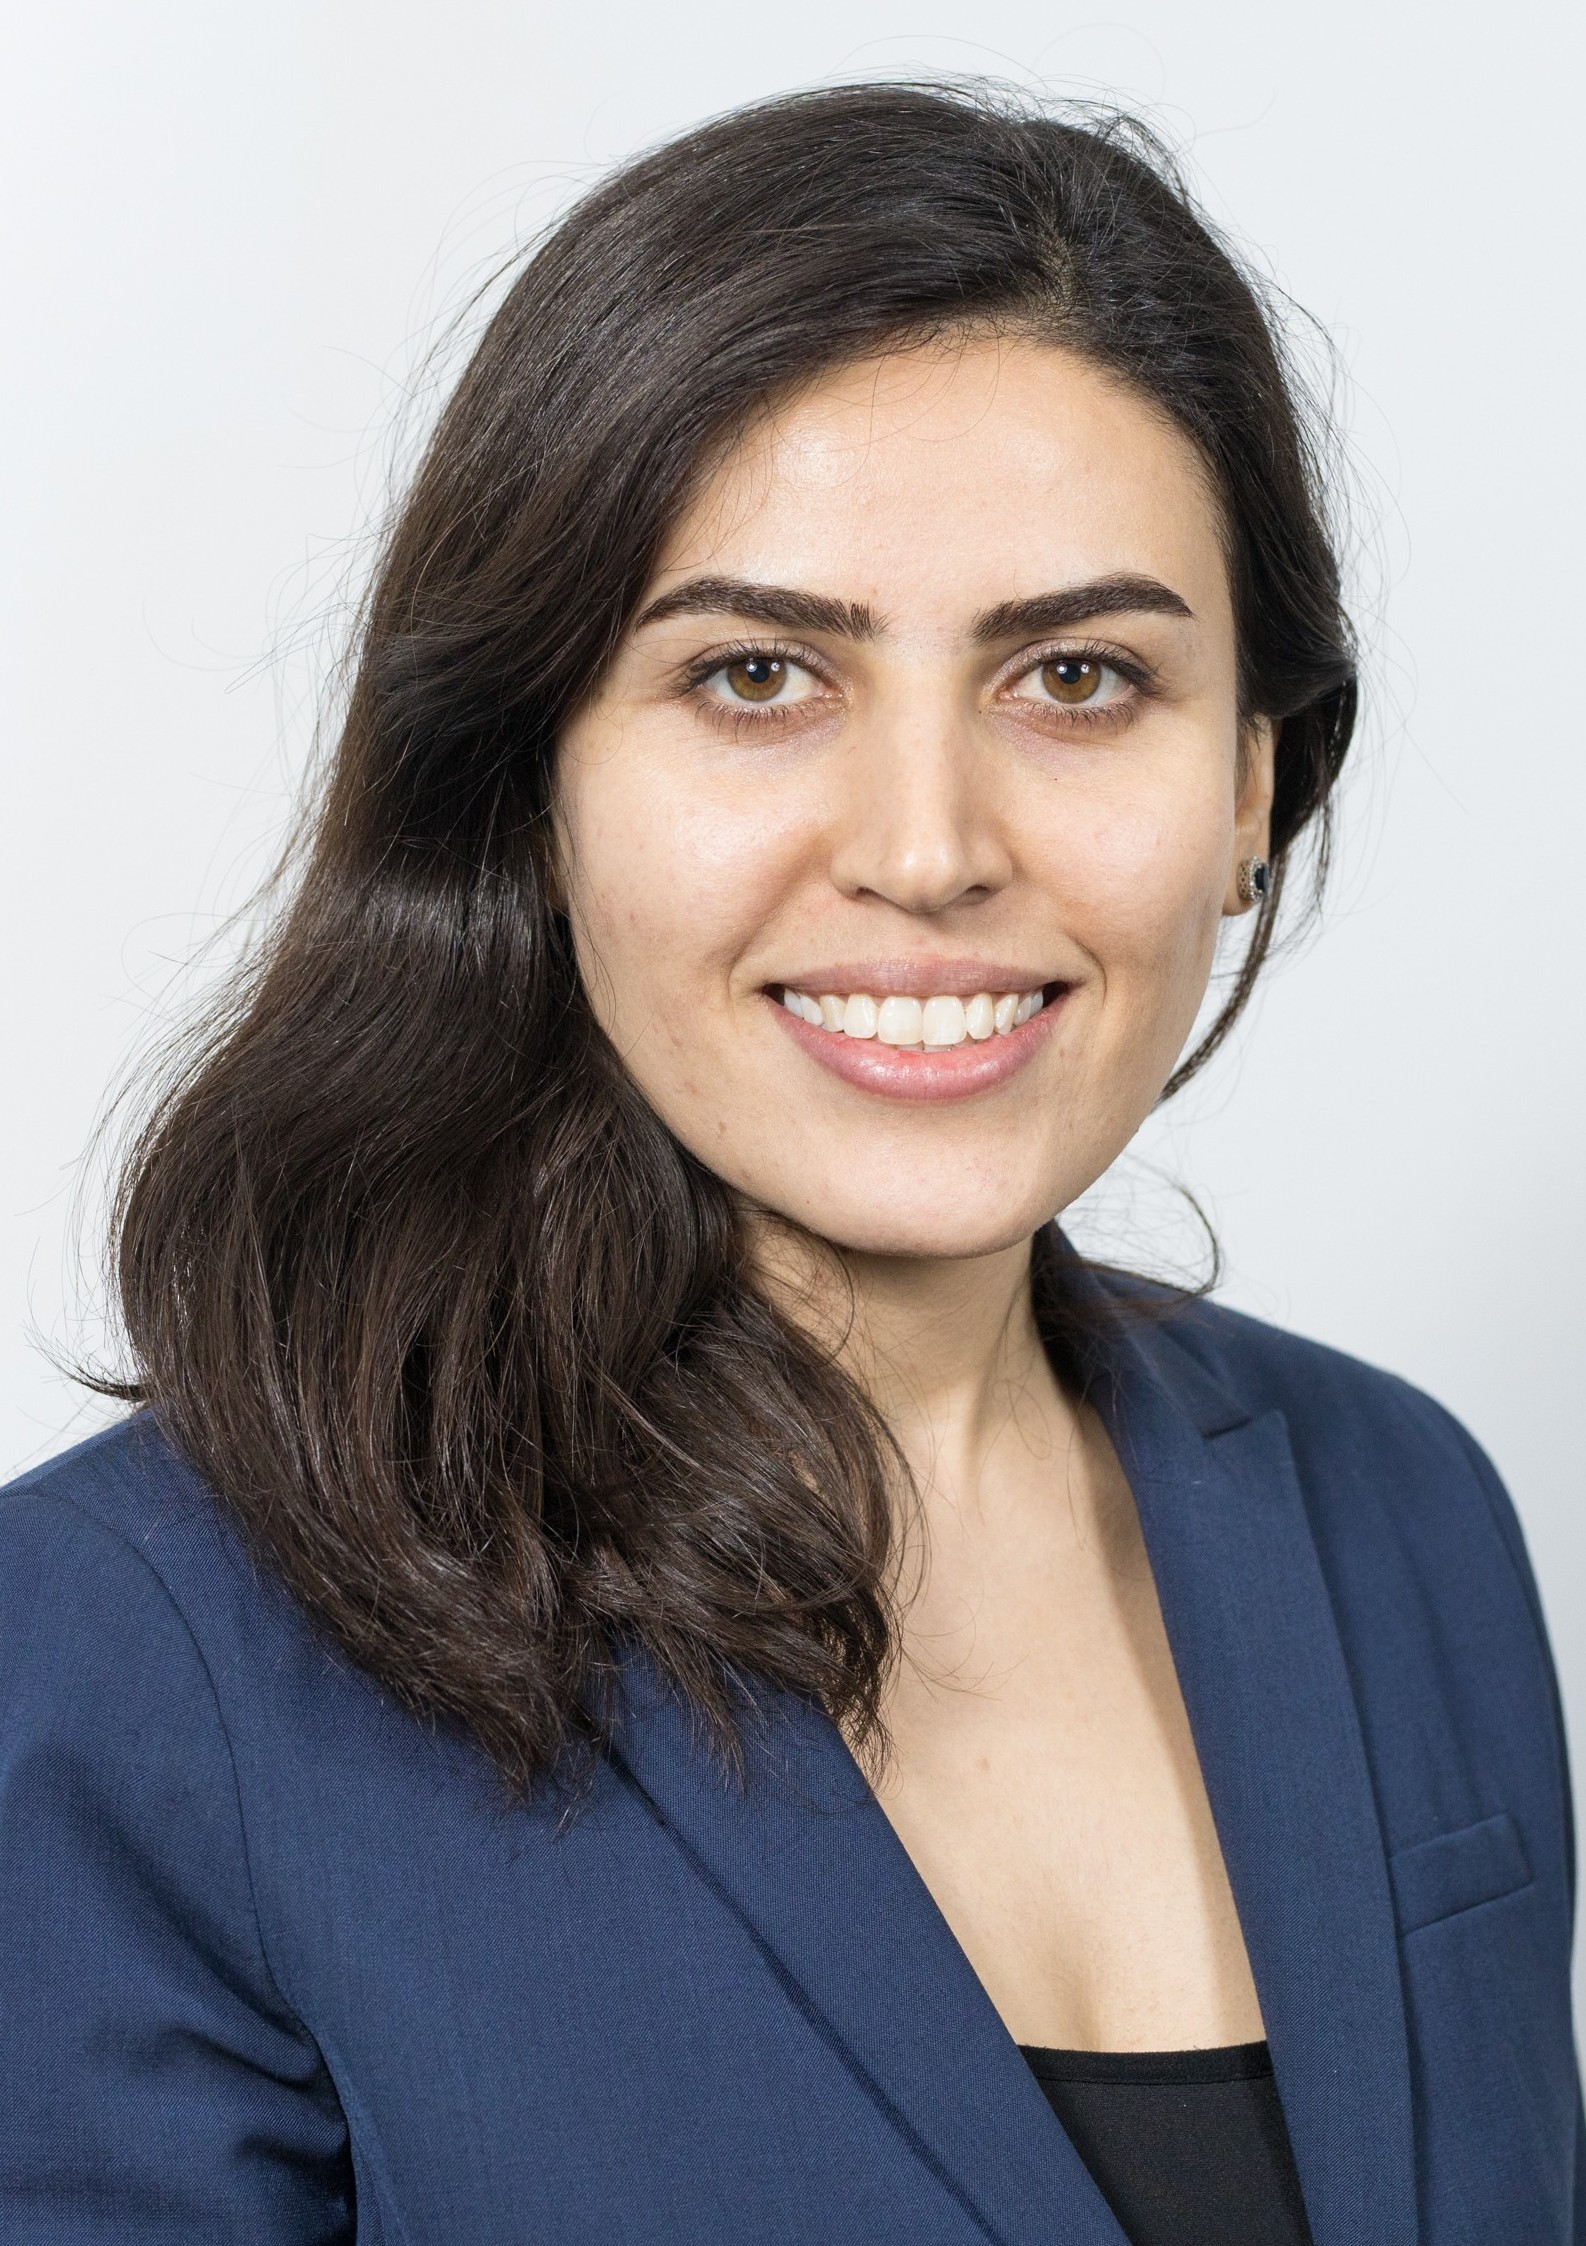
\includegraphics{plots/Mina.jpg}}

  \end{figure}
  
\end{frame}


\begin{frame}  {Emilio Dorigatti, M.Sc.}

 I am Ph.D. Researcher at the Chair of Statistical Learning and Data Science.
    \begin{itemize}
      \item Double Master's degree (from the Technical University of Eindhoven and from the Royal Institute of Technology, Stockholm) in Data Science obtained through the EIT Digital Master School, as well as a minor degree in Innovation and Entrepreneurship.
      \item B.Sc. in Computer Science
    \end{itemize}
    
  \begin{figure}
    \centering
      \scalebox{0.25}{\includegraphics{plots/dorigatti.jpg}}

  \end{figure}
  
\end{frame}



\section{Course Roadmap}

\begin{frame}  {Content Table}

\begin{enumerate}
\item Introduction, Overview, and a Brief History of Deep Learning

\item Deep Forward Neural Network, Gradient Descent, Backprop, Hardware and Software

\item Regularization of NNs, Early Stopping

\item Dropout and Challenges in Optimization

\item Advanced Optimization

\item Activation Function and Initialization

\item Convolutional Neural Network, CNN Variants, Applications

\item  Modern CNN and Overview of some applications

\item Recurrent Neural Network

\item Modern RNN and Applications

\item Deep Unsupervised Learning

\item Autoencoders, AE Regularization and Variants

\item Manifold Learning

\item Deep Generative Models, VAE, GANs

\end{enumerate}
    
  
\end{frame}


\section{Deep Learning Application}

\begin{frame}  {Applications of Deep Learning}
  \begin{figure}
    \centering
      \scalebox{1}{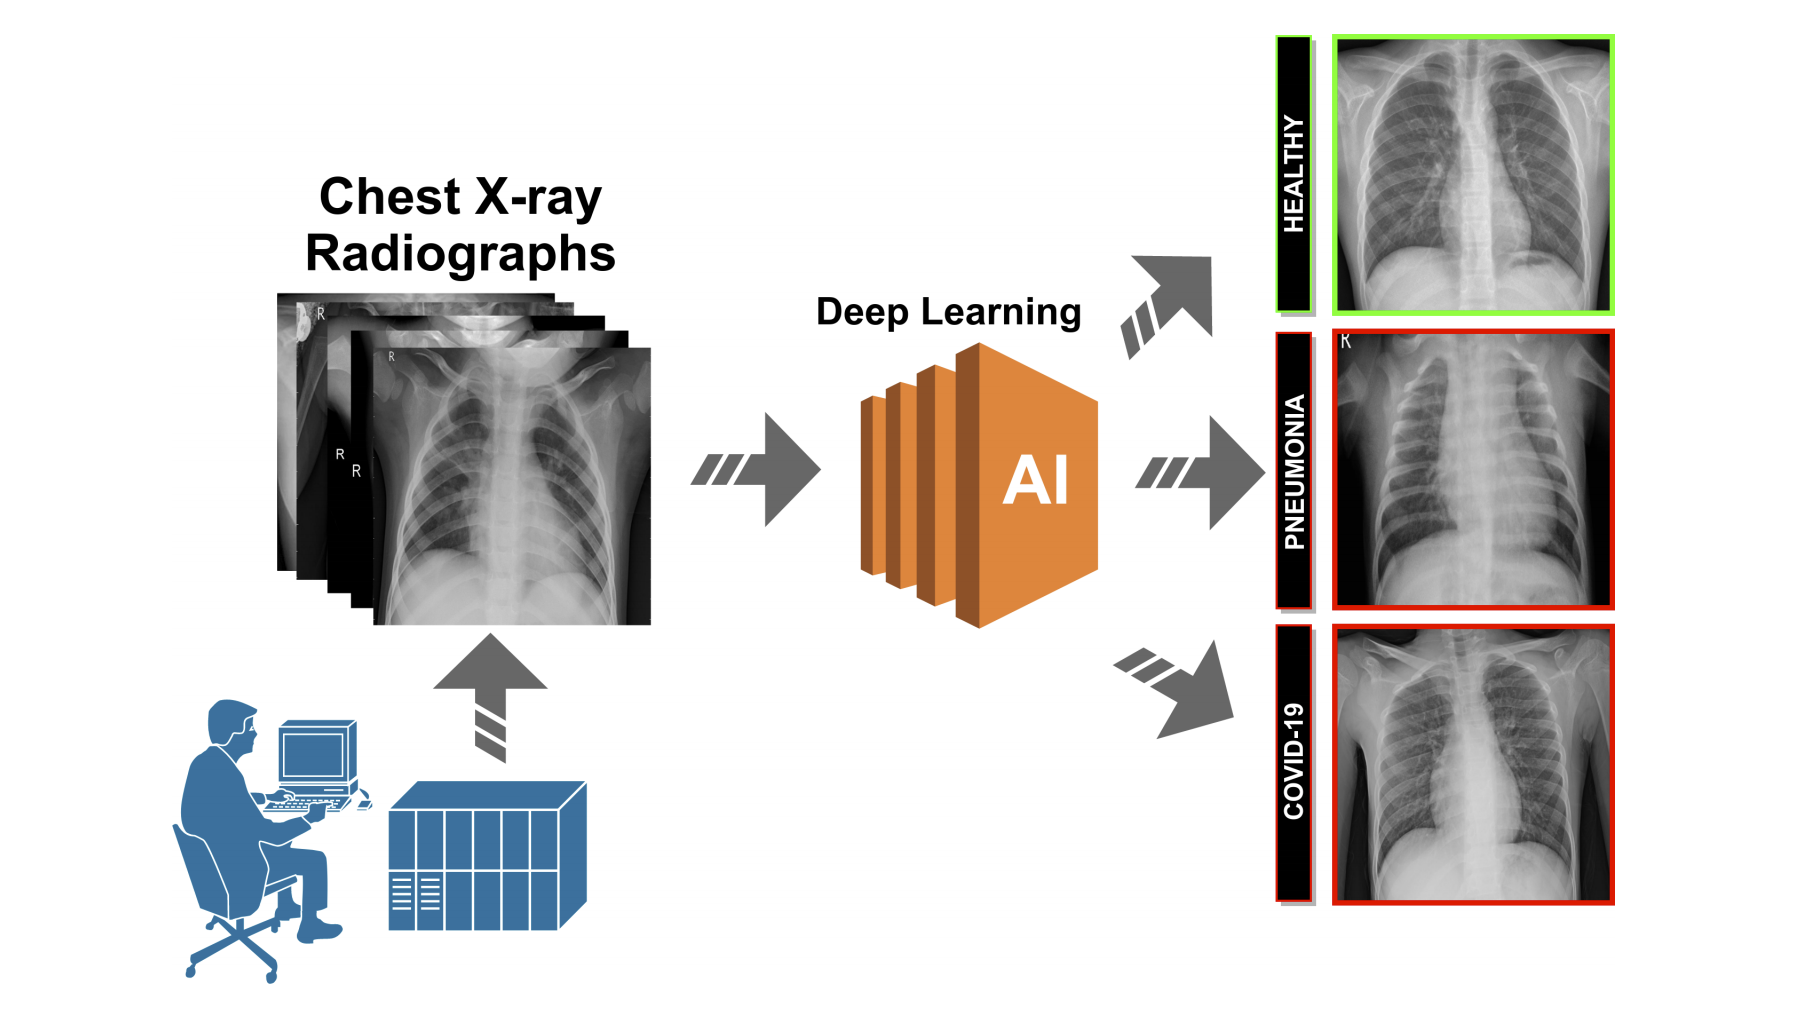
\includegraphics{plots/covid19.png}}

  \end{figure}
  \hspace{1cm} \textbf{Impact on healthcare: Covid-19 diagnosis}\\ \hspace{1cm}(Source: CITIC Research Center)
\end{frame}

\begin{frame} {Applications of Deep Learning}
  \begin{figure}
    \centering
      \scalebox{0.95}{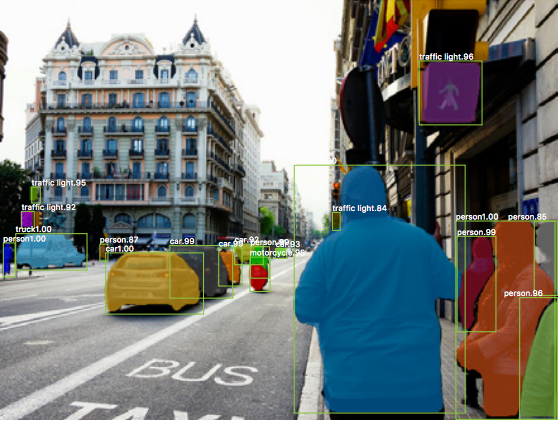
\includegraphics{plots/maskrcnn.png}}
  \end{figure}
   \hspace{3cm}     \textbf{Machine Vision} (Credit: Kaiming He)
\end{frame}

\begin{frame}  {Applications of Deep Learning}
  \vspace{5mm}
  \begin{figure}
    \centering
      \scalebox{1}{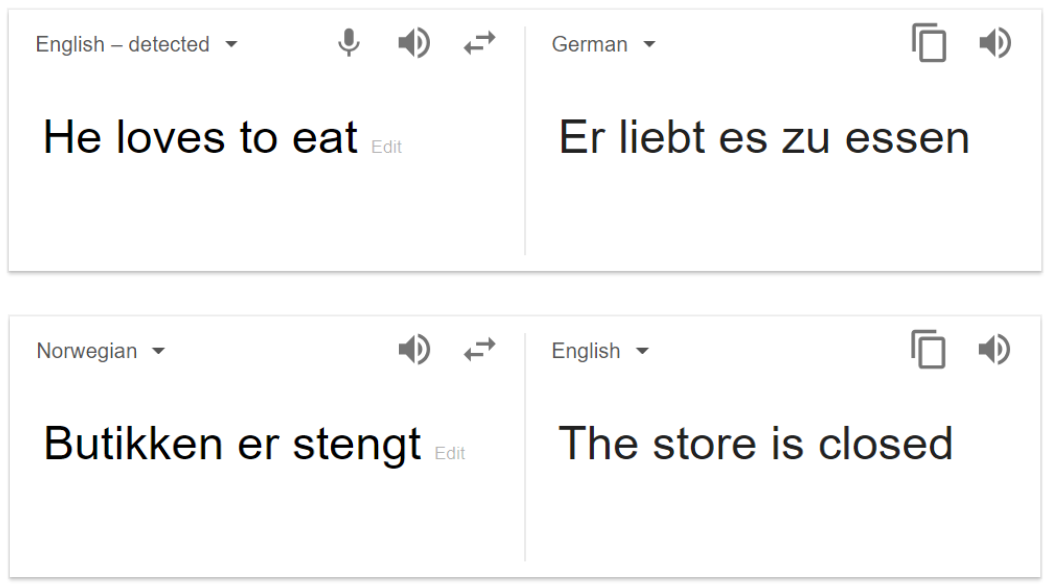
\includegraphics{plots/nmt.png}}
  \end{figure}
    \hspace{4cm} \textbf{Machine Translation}
\end{frame}

\begin{frame}  {Applications of Deep Learning}
  \begin{figure}
    \centering
      \scalebox{1}{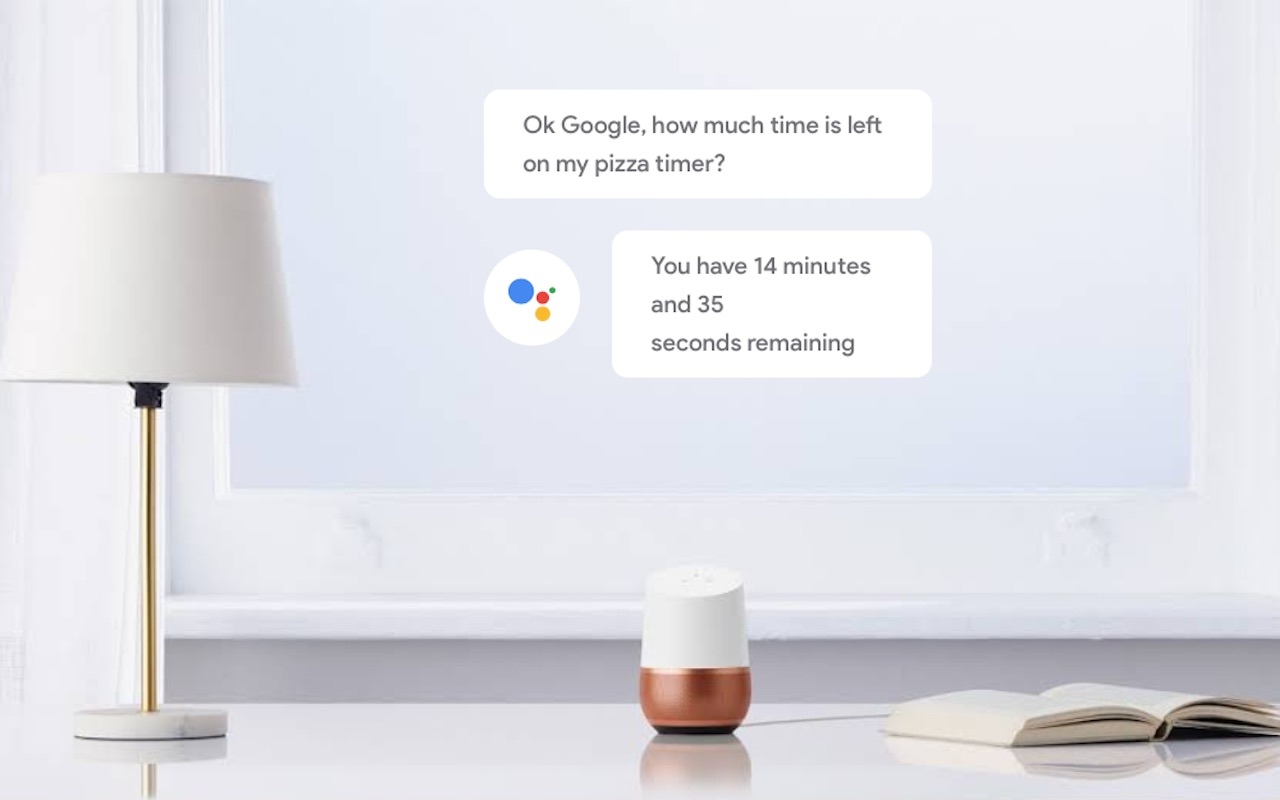
\includegraphics{plots/speech_goog.jpg}}

  \end{figure}
  \hspace{1cm} \textbf{Speech Recognition and Generation} (Source: Google)
\end{frame}

\begin{frame}  {Applications of Deep Learning}
  \begin{figure}
    \centering
      \scalebox{1}{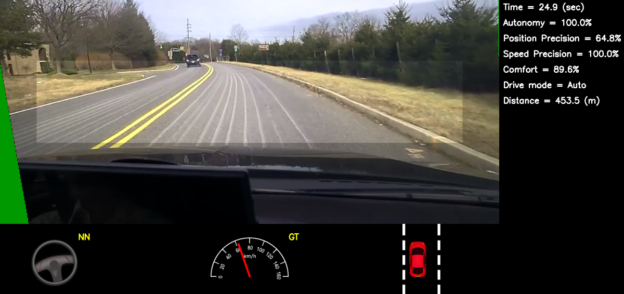
\includegraphics{plots/nvidia_self_driving_sim.png}}

  \end{figure}
  \hspace{1cm} \textbf{End-to-End Deep Learning for Self-Driving Cars} (Source: Nvidia)
\end{frame}

%%%%%%%%%%%%%%%%%%%%%%%%%%%%%%%%%%%%%%%%%%%%%%%%%%%%%%%%%%%%%%%%%%%%%%%%%%%%%%%%%%%%%%%%%%%%%%%%%%%
%%%%%%%%%%%%%%%%%%%%%%%%%%%%%%%%SINGLE NEURON%%%%%%%%%%%%%%%%%%%%%%%%%%%%%%%%%%%%%%%%%%%%%%%%%%%%%%
%%%%%%%%%%%%%%%%%%%%%%%%%%%%%%%%%%%%%%%%%%%%%%%%%%%%%%%%%%%%%%%%%%%%%%%%%%%%%%%%%%%%%%%%%%%%%%%%%%%

% \begin{frame} {Intro to ML 1*}
%   \begin{itemize}
%     \item The universe, laws and patterns
%     \item Approximate the function f
%     \item Learn from experience
%   \end{itemize}
% \end{frame}
% 
% \begin{frame} {Intro to ML 2*}
%   \begin{itemize}
%     \item SL vs UL
%     \item Features
%     \item labels, regression, classification
%   \end{itemize}
% \end{frame}
\section{What is Machine Learning? }

\begin{vbframe}{What is Machine Learning? }

\vspace{2cm}

\begin{center}
  \fontsize{13pt}{13pt}\selectfont
 % Machine Learning is a method of teaching computers to make predictions based on some data.
  A computer program is said to \textbf{learn} from experience E with respect to some task T and some performance measure P, if its performance on T, as measured by P, improves with experience E. \\
  \begin{footnotesize}
  \emph{Tom Mitchell, Carnegie Mellon University, 1998}
  \end{footnotesize}
\end{center}

\framebreak 

All machine learning algorithms consist of three key components:
  \begin{itemize}
    \item \textbf{Hypothesis space}:
    \begin{itemize}
      \item This is basically the search space of the algorithm. 
      \item It is the predefined set of functions from which the algorithm picks a function/model that is the best fit to the data.
    \end{itemize}
    \vspace{4mm}
    \item \textbf{Risk}:
    \begin{itemize}
      \item A metric by which to evaluate models in the hypothesis space.
      \item The model returned by the algorithm must perform well on \textit{unseen} data.
    \end{itemize}
    \vspace{4mm}
    \item \textbf{Optimizer}:
      \begin{itemize}
        \item A method/algorithm to find the \enquote{right} model.
      \end{itemize}
  \end{itemize}

\end{vbframe}

\section{Deep Learning }


\begin{frame} {Deep Learning}

\vspace*{-0.5cm}

\begin{center}
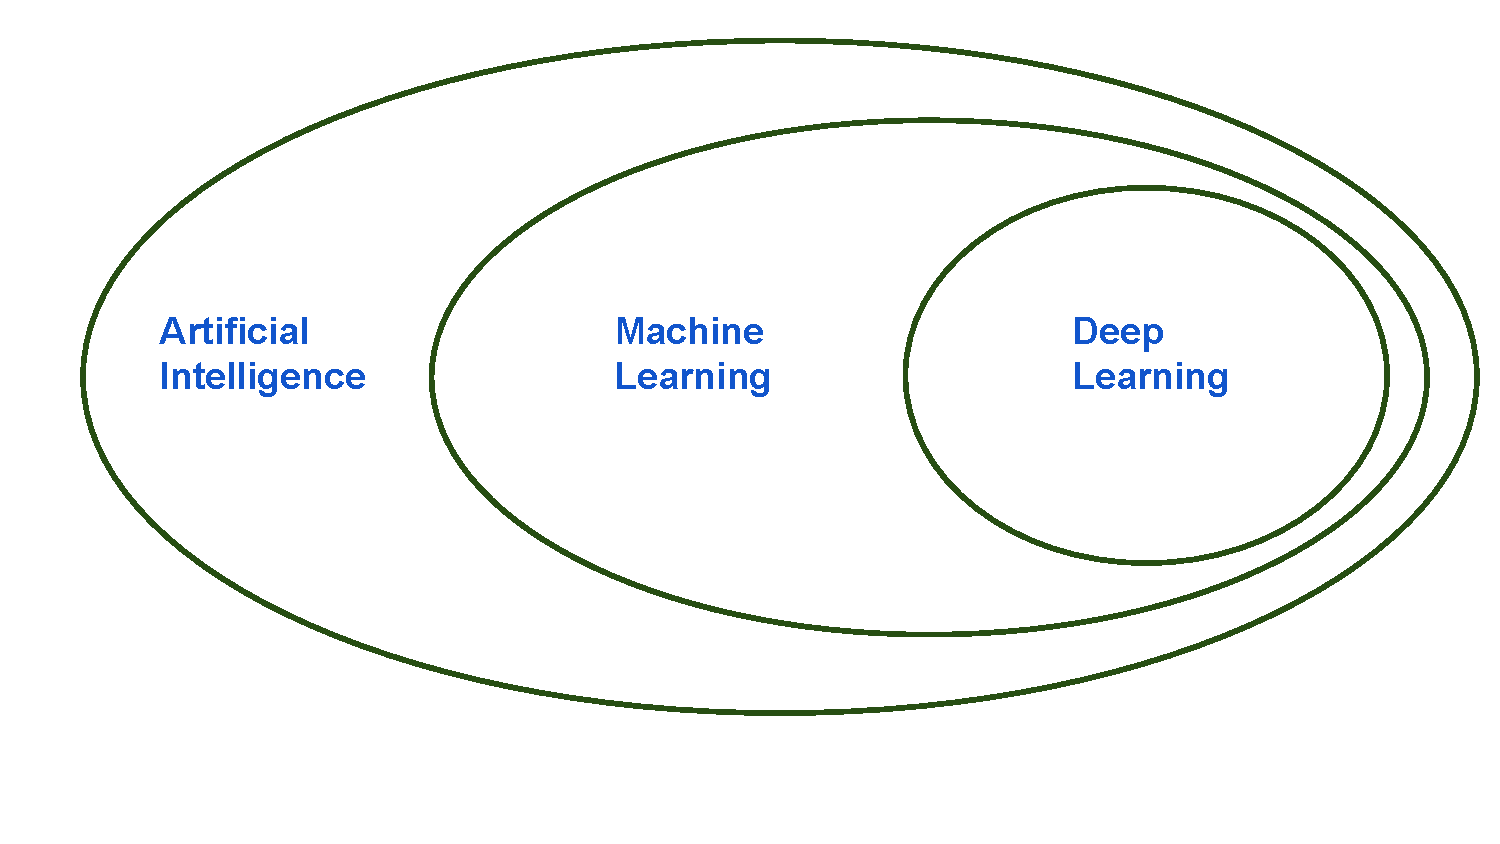
\includegraphics[width=0.8\textwidth]{plots/learning.pdf}
\end{center}

\vspace*{-1cm}

  \begin{itemize}
    \item (Deep) neural networks are fundamentally a special kind of hypothesis space (\textit{very}) loosely inspired by the organisation of neurons in biological brains.
    \item This lecture is about the nature of this hypothesis space.
    \item Some (important!) added tricks related to optimization will be covered in later lectures.
  \end{itemize}
\end{frame}

\endlecture
\end{document}